% ===================================
% CODICE LaTeX PER GRAFICI E TABELLE
% Tesi GDO - Capitoli 1 e 2
% ===================================
% filepath: c:\Users\saint\tesi\nuovi grafi 1 e 2.tex
\documentclass[border=10pt]{standalone}
% Pacchetti necessari
\usepackage[utf8]{inputenc}
\usepackage[T1]{fontenc}
\usepackage{amsmath}
\usepackage{amssymb}    
\usepackage{graphicx}
\usepackage{caption}
\usepackage{subcaption} % Per sottotitoli nelle figure
% Preambolo necessario:
\usepackage{tikz}
\usepackage{pgfplots}
\usepackage{booktabs}
\usepackage{multirow}
\pgfplotsset{compat=1.17}
\usetikzlibrary{pgfplots.polar}
\begin{document}
% FIGURA 2.4: Confronto Costi Compliance
%\begin{figure}[h]
\centering
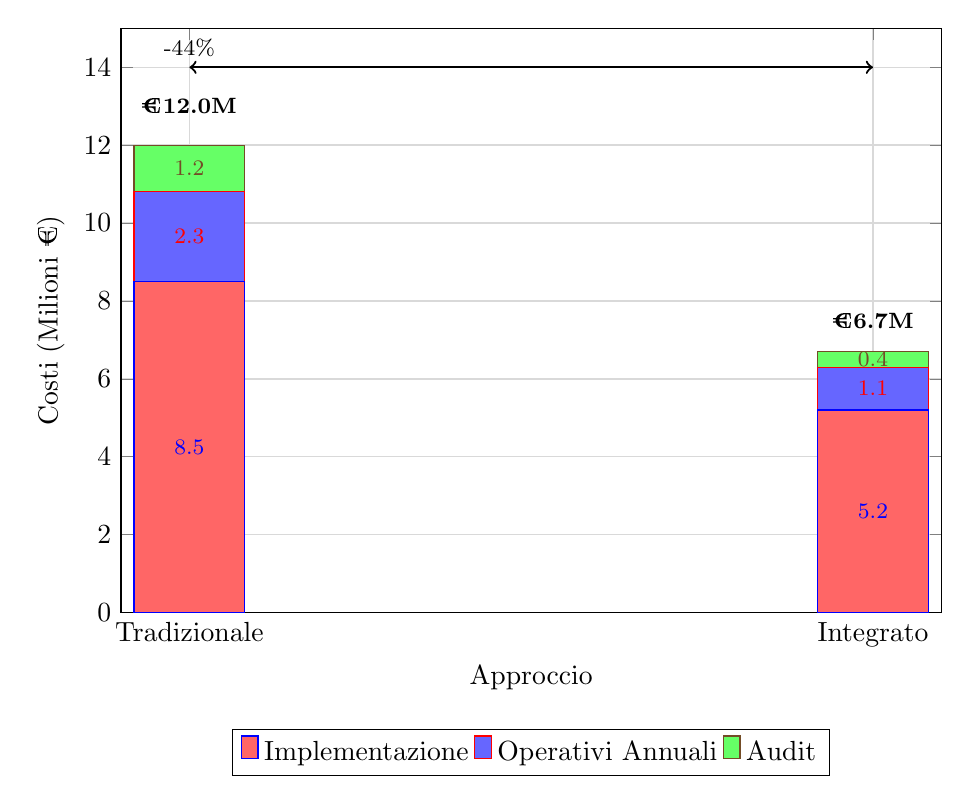
\begin{tikzpicture}
\begin{axis}[
    ybar stacked,
    width=12cm,
    height=9cm,
    ylabel={Costi (Milioni €)},
    xlabel={Approccio},
    symbolic x coords={Tradizionale,Integrato},
    xtick=data,
    bar width=40pt,
    ymin=0,
    ymax=15,
    legend style={at={(0.5,-0.2)},anchor=north,legend columns=3},
    nodes near coords,
    every node near coord/.append style={font=\footnotesize},
    grid=major,
    grid style={line width=0.5pt, draw=gray!30}
]

\addplot+[ybar,fill=red!60] coordinates {(Tradizionale,8.5) (Integrato,5.2)};
\addplot+[ybar,fill=blue!60] coordinates {(Tradizionale,2.3) (Integrato,1.1)};
\addplot+[ybar,fill=green!60] coordinates {(Tradizionale,1.2) (Integrato,0.4)};

\legend{Implementazione,Operativi Annuali,Audit}

% Etichette totali
\node at (axis cs:Tradizionale,13) {\footnotesize \textbf{€12.0M}};
\node at (axis cs:Integrato,7.5) {\footnotesize \textbf{€6.7M}};

% Risparmio percentuale
\draw[<->,thick] (axis cs:Tradizionale,14) -- (axis cs:Integrato,14);
\node at (axis cs:Tradizionale,14.5) {\footnotesize -44\%};

\end{axis}
\end{tikzpicture}
\end{document}